\subsubsection{Start \& Stop Condition}
\label{chap:Back_I2C_Protocol_Start_Stop}

Every bus transaction begins with a START condition (ST). A START condition 
is defined as a HIGH-to-LOW transition on SDA while SCL remains HIGH. 
Conversely, a STOP condition (SP) is defined as a LOW-to-HIGH transition on SDA 
while SCL remains HIGH. Both START and STOP conditions are always generated 
by the master.

Once a START condition occurs, the bus is considered busy; it becomes free 
again a specified time after a STOP condition. If the master issues a repeated 
START instead of a STOP, the bus remains busy, and the master can initiate a new 
transaction without releasing control of the bus.

\begin{figure}[H]
    \centering
    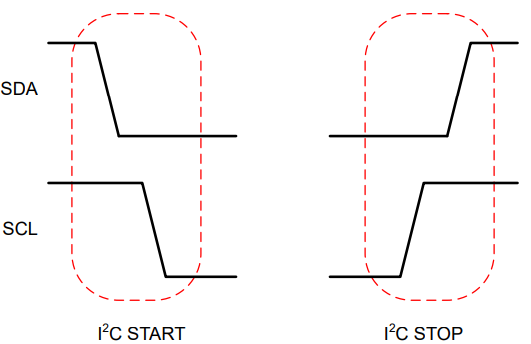
\includegraphics[width=0.4\textwidth]{Resources/Imagenes/start_&_Stop.png}
    \caption{Start \& Stop Conditions}
    \label{fig:Start_/&_stop}
\end{figure}
